\chapter{Functional schema}

% sezione velocemente descrittiva del datapath
\section{Datapath}

% schema del datapath, possibilmente numerato 
\begin{figure}[ht]
	\centering
	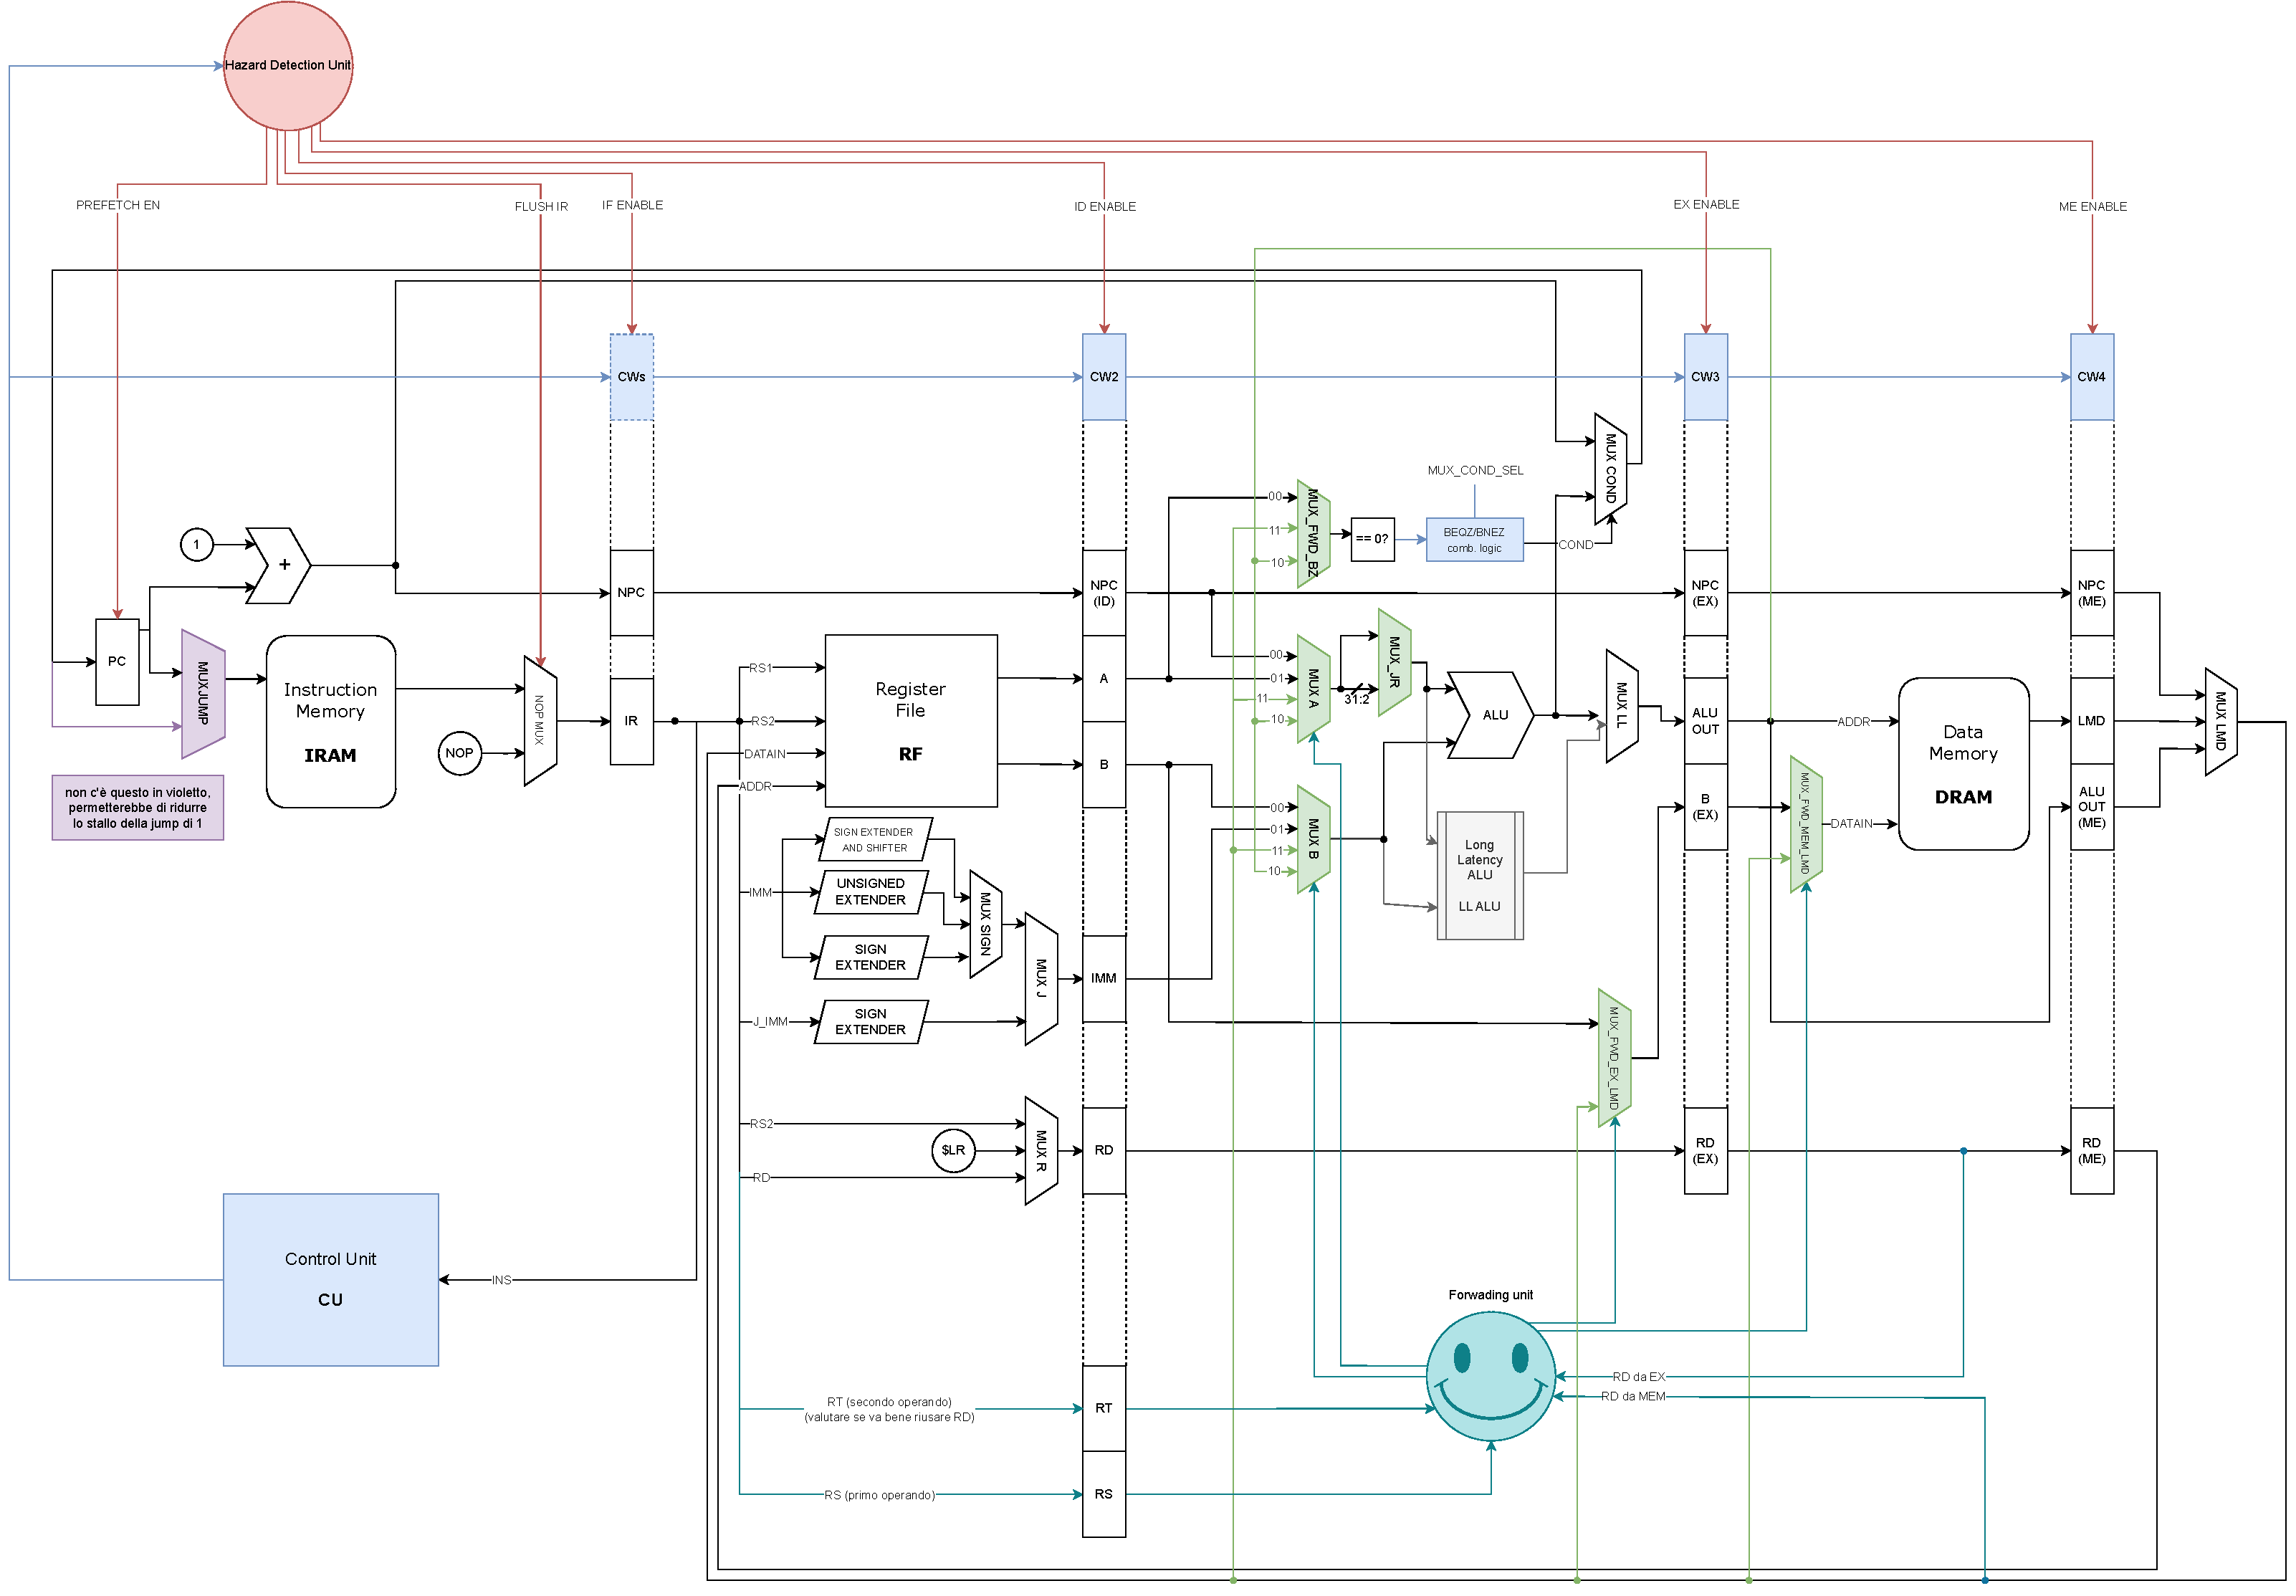
\includegraphics[width=\textwidth]{chapters/figures/datapath.pdf} 
	\caption{sus}
	\label{fig:datapath}
\end{figure}


% sezione sulle singole unità funzionali del datapath, presentate come blackbox e successivamente con l'implementazione interna, questo per ognuna di esse
\section{Functional blocks}
\subsection{Control unit}
% TODO schema della control unit? si dovrebbe vedere come viene effettivamente sintetizzata
% CHE CAZZO È CW_FROM_MEM DIO CANE
The Control Unit is in charge of managing the datapath throughout its stages. Given an instruction from IR, it generates the corresponding control word that manages the various registers, MUXes and other control signals in the datapath. It also receives a block of \emph{STALL} signals from the HDU (Hazard Detection Unit) that instructs the CU on when to stall the pipeline in case of data hazards. % solo data hazards?



% non so se questa cosa è effettivamente vera, è una LUT alla fine
It is implemented as an hybrid between an hardwired and a microcoded CU, with two processes that simply associate every instruction with a given control word and every ALU opcode with the corresponding operation, plus a process that manages the transition between every stage taking into consideration the \emph{STALL} signals from the HDU.

\subsection{Register file}
The register file included in the DLX contains 32 registers, each of word size equal to 32 bits. Following the MIPS ISA, register $ \mathit{R0} $ has its value hardcoded to 0 and register $ \mathit{R31} $ is the \emph{Link Register} used for returning from subroutines.
% following the MIPS isa


It has been chosen to be a Double-read/Single-write type, as in: on every clock cycle, the register file can output the values of two registers at the time by providing addresses on ports \emph{ADD\_RD1} and \emph{ADD\_RD2} and requesting reads on ports \emph{RD1} and \emph{RD2}; a write can be made by setting an address on \emph{ADD\_WR} and a word on port \emph{DATAIN}. Requested registers output their value on ports \emph{OUT1} and \emph{OUT2}. 
% CRISTO with the corresponding two ports for address selection and data out for reading and single port for address and data in for writing, plus 

\subsection{ALU}
% TODO aggiungere schema a blocchi dell'ALU
% scrivi anche come sono mussati gli ingressi
% The ALU can pick its inputs from a moltitude of sources 
The ALU of the DLX operates on two inputs: \emph{DATA1} and \emph{DATA2}. It can obtain them from a multitude of sources, namely: 
\begin{itemize}
	% Gli input muxati possono essere non solo i registri di ingresso A e B ma anche forwardati da altri stage, essere un immediato etc.
	\item from the register file, through 2 stage registers \emph{A} and \emph{B};
	\item from the program counter, necessary for address computations in branching and jump instructions;
	\item from the instructions themselves, immediate values via the instruction register after the appropriate transformations;
	\item from the ALU itself, and in general from other stages' outputs through MUXes controlled by the forwarding unit.
\end{itemize}
% La grandezza è configurabile ma è settata di default a 32 bits IIRC


The function to be computed on the operands is selected by a third input \emph{FUNC} that receives a code representing it and the result is sent to the output \emph{OUTALU}. A list of currently implemented functions follows. The implementation of each operation is behavioural unless specified otherwise. 

% TODO fix indentations
\subsubsection{Addition}
$ \mathit{ALUOUT} = \mathit{DATA1} + \mathit{DATA2} $

A P4 adder is present inside the ALU to perform additions. Further details on its implementation together with the VHDL description are included in lab 2's zip file.

\subsubsection{Subtraction}
$ \mathit{ALUOUT} = \mathit{DATA1} - \mathit{DATA2} $


The P4 adder is also used for subtractions, by means of negating one of  the inputs and setting the carry-in input of the adder to 1.

\subsubsection{Multiplication}
% TODO aggiungere simbolo del troncamento a word size
$ \mathit{ALUOUT} = \mathit{DATA1} \cdot \mathit{DATA2} $


Multiplication is executed on the operands fully but the result is still word size: the most significant half of the computed value is discarded.


Initially, the multiplication operation was to be delegated to a long latency ALU, with this implementation just being a placeholder. However the group decided to focus on more difficult to implement features, leaving no time for description and testing of an LL ALU.

\subsubsection{AND}
$ \mathit{ALUOUT} = \mathit{DATA1} \wedge \mathit{DATA2} $

\subsubsection{OR}
$ \mathit{ALUOUT} = \mathit{DATA1} \lor \mathit{DATA2} $

\subsubsection{XOR}
$ \mathit{ALUOUT} = \mathit{DATA1} \oplus \mathit{DATA2} $

\subsubsection{Logical Shift Left}
$ \mathit{ALUOUT} = \mathit{DATA1} \ll \mathit{DATA2} $

\subsubsection{Logical Shift Right}
$ \mathit{ALUOUT} = \mathit{DATA1} \gg \mathit{DATA2} $

\subsubsection{Set equal}
$ \mathit{if (DATA1 == DATA2) \: then} \: \mathit{ALUOUT} = 1 \: \mathit{else} \: 0 $

\subsubsection{Set not equal}
$ \mathit{if (DATA1 \neq DATA2) \: then} \: \mathit{ALUOUT} = 1 \: \mathit{else} \: 0 $

\subsubsection{Set greater than or Equal (signed and unsigned)}
$ \mathit{if (DATA1 \geq DATA2) \: then} \: \mathit{ALUOUT} = 1 \: \mathit{else} \: 0 $

\subsubsection{Set greater than (signed and unsigned)}
$ \mathit{if (DATA1 > DATA2) \: then} \: \mathit{ALUOUT} = 1 \: \mathit{else} \: 0 $

\subsubsection{Set less than or Equal (signed and unsigned)}
$ \mathit{if (DATA1 \leq DATA2) \: then} \: \mathit{ALUOUT} = 1 \: \mathit{else} \: 0 $

\subsubsection{Set less than (signed and unsigned)}
$ \mathit{if (DATA1 < DATA2) \: then} \: \mathit{ALUOUT} = 1 \: \mathit{else} \: 0 $

\subsection{Hazard detection unit}
The Hazard Detection Unit takes care of detecting data and control hazards in the pipeline and successively dispatching stage enable (or STALL, as written in the CU subsection) signals to the CU for indication on where and for how many stages to stall for. It does so by progressively checking for hazardous conditions in a process starting from IRAM and DRAM readiness, then for branches (assuming not taken), jumps and loads from memory giving precedence, in case of instructions of the same type, to instructions currently found in the execute stage. If no hazardous condition is found, a STALL\_CLEAR signal is sent out.

\subsection{Forwarding unit}
The Forwarding Unit takes as input a subset of the control signals sent by the CU and of the register selection codes (not the values inside the registers themselves). Given those, it detects favourable conditions for source and destination registers between stages of the pipeline and if they match it forwards operands where they are needed by changing selection signals for the appropriate MUXes and skipping the write-back stage.